\subsection{\href{http://www.nanocut.com/}{Nanocut}}
   \hypertarget{subsec:nanocut}
   Working for Nanocut company at Moldova I've developed a PMSM (\textit{permanent magnet synchronous motor}) servo motor controller using a Texas Instruments development board with a C2000 real-time microcontroller.
   I've implemented a torque, speed and position closed loop control algorithms using a relative optical encoder as a feedback.
   I've implemented a FOC vector control method using Clarke / Parke transforms and three nested PID’s.
   This work will be the hardware and firmware base for a new generic servo driver for using in all the company's machines.
   Figure \ref{fig:nanocut_electronica} shows the hardware tools and the algorithms implemented.
     \begin{figure}
      \begin{center}
         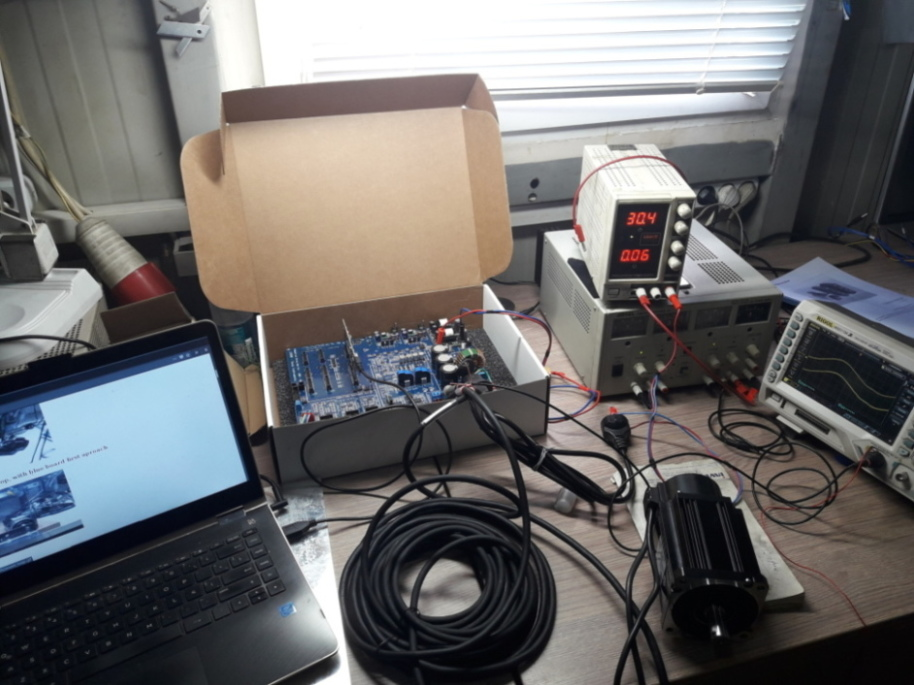
\includegraphics[width=0.3\textwidth]{nanocut1.jpg}
         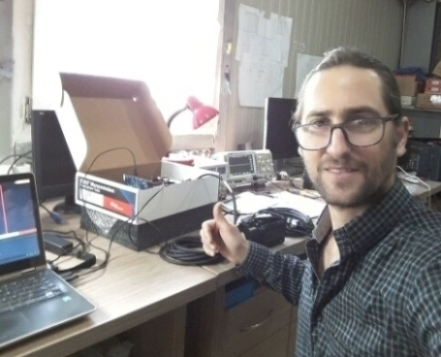
\includegraphics[width=0.3\textwidth]{nanocut2.jpg}
         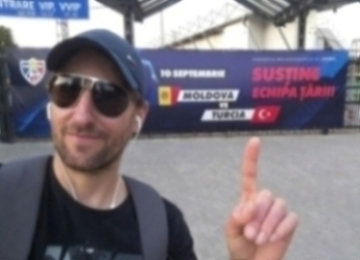
\includegraphics[width=0.3\textwidth]{nanocut3.jpg}
      \end{center}
      \caption{Development tools and algoritm output plots of the PMSM servo driver}
      \label{fig:nanocut_electronica}
   \end{figure}
   Figure \ref{fig:nanocut_mecanica} shows the prototype running at Nanocu's labs.
  \begin{figure}
      \begin{center}
         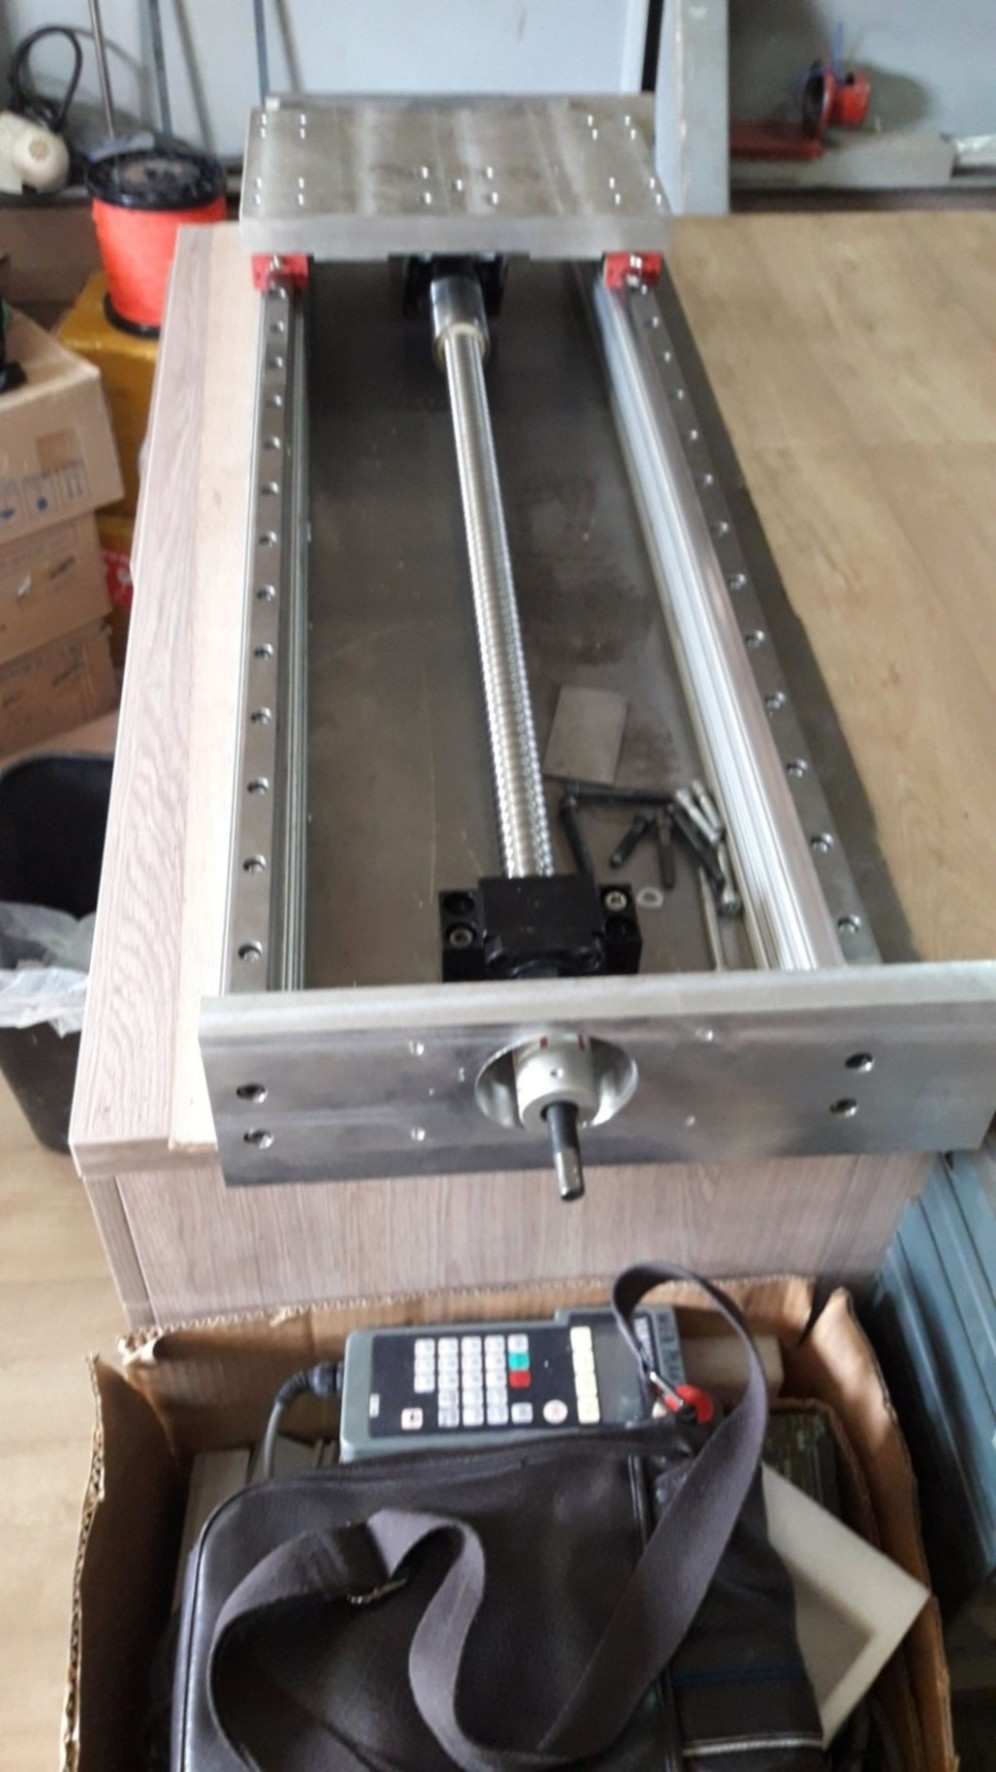
\includegraphics[width=0.3\textwidth]{nanocut4.jpg}
         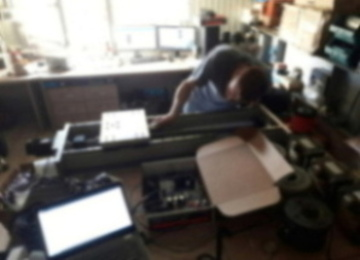
\includegraphics[width=0.3\textwidth]{nanocut5.jpg}
         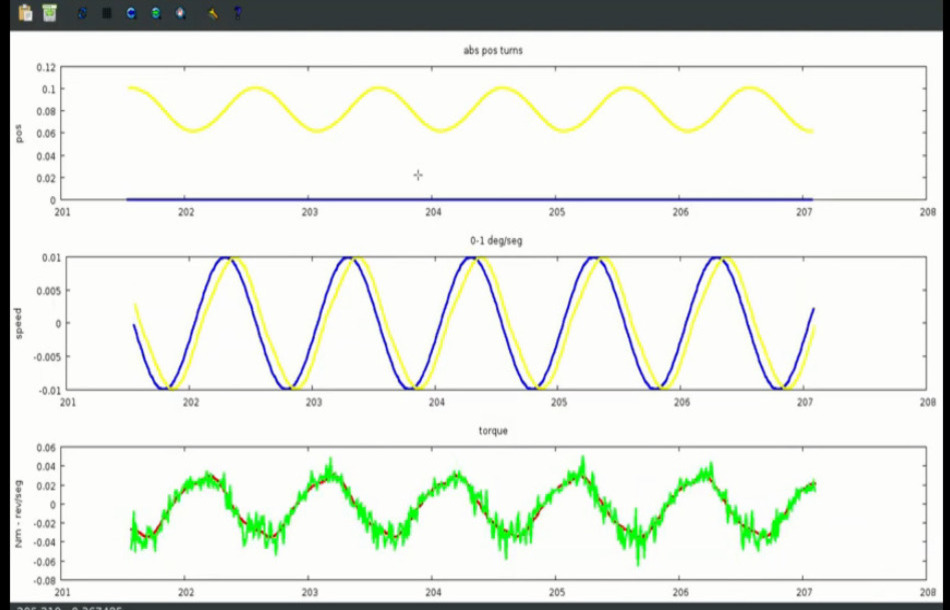
\includegraphics[width=0.3\textwidth]{nanocut6.jpg}
      \end{center}
      \caption{Mechanical prototype used fot the PMSM algoritm test, torque, speed and position}
      \label{fig:nanocut_mecanica}
   \end{figure}

